\section{Practice}
\label{sec:experiments}

This section will provide the implementation details of the theory part (Section \ref{sec:theory}). The algorithm is implemented in C ++ and makes use of the CGAL library (\url{https://www.cgal.org}). 
Then, given the implementation, experimental setups will be introduced. The experimental setup will include some basic test polygons to check the correct execution of the algorithm. We will also observe the behaviour of the algorithm and emphasise the importance of each of the heuristics used. Lastly, we will showcase the fragility and importance of hyperparameters.

Polygons used:
- 2 guards
- random
- love
- comb
- corridor

For every heuristic:
- show how each polygon behaves when turning it off

Try to see if the comb polygon scales

\subsection{Heuristics}
In this subsection we will observe the role played by each of the heuristics used. We will additionally notice how different heuristics are more relevant for different types of polygons. In order to do so, we will run the program with all of the heuristics but one, for each of the heuristics. By analysing the difference in movement for each of the guards', we will be able to assess the influence every heuristic has on each type of polygon.

We will use fixed hyperparameters for all the runs. This will allow us to focus on the differences between the heuristics. Later in this section we will also discuss the actual hyperparameter choice. As such, we will use a momentum past weight $\gamma = 0.8$ and pull attraction $\beta = 1$. The learning rate will be varied per polygon and type of experiment. This choice is due to the fragility of the algorithm implementation and will be explained later in this section.

\subsubsection{Without Momentum}
In this section we will discuss the impact momentum has on the overall behaviour of the algorithm. As introduced in Section \ref{sec:momentum}, momentum takes into account the position history of the guards. In this way, the overall trajectory of a guard is smoothened out.

A suggestive way to observe this is with the arbitrary polygon from Figure \ref{fig:random}. The polygon requires a minimum of 3 guards to be fully seen. For this reason, we will run the algorithm with only 3 guards.

\begin{figure}[h!]
    \centering
    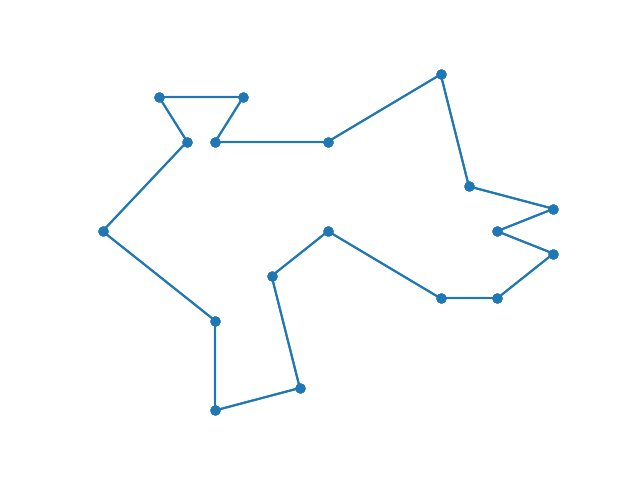
\includegraphics[width = 0.5\textwidth]{experiments/random.png}
    \caption{Arbitrarily shaped polygon.}
    \label{fig:random}
\end{figure}

We will compare how the guards move when we are using all the heuristics to when we are not using momentum. The guards will have a learning rate $\alpha = 0.2$. They will start at the same fixed position in both cases.

Figure \ref{fig:no_momentum} displays the area seen per iteration for the arbitrary polygon Both the total area seen and the individual area seen by each are shown. Starting with almost the whole area seen, the guards are eventually optimally placed in a position from which the whole polygon is seen. Nonetheless, using momentum clearly makes a difference in Subfigure \ref{fig:no_momentum1}, than when not using it in Subfigure \ref{fig:no_momentum2}. Using momentum allows the overall seen area to keep a steady trajectory towards its maximum. Additionally, guards quickly find their optimum in only 4 iterations, without many oscillations. In Subfigure \ref{fig:no_momentum2} however we can observe how the total area fluctuates. The guards also display large jumps close to iterations 5 and 20. These jumps cause the overall progress towards the optimum to be less stable. For example, when guard 2 has a sudden drop in the area it sees around iteration 5, the total area seen naturally drops as well, and only recovers after iteration 20, when guard 0 makes another large jump. This behaviour also suggests that the movement of one guard can heavily influence others, resulting in a noisy behaviour and in a higher number of iterations.
% Subfigure \ref{fig:no_momentum1} displays a more smoothened out trajectory for each guard. 
Therefore, it becomes clearer how momentum allows the smoothening of noisy guard movements. Additionally, we reckon that because guards are holding a steadier trajectory, they are more likely to achieve the optimum in less iterations (in this example, 3). When not using momentum, the number of iterations increases substantially to 24. Momentum thus is a crucial improving heuristic to our whole algorithm, both in speedup as well as in the smootheness of the process.

\begin{figure}[h!]
    \centering
    \begin{subfigure}{0.45\textwidth}
        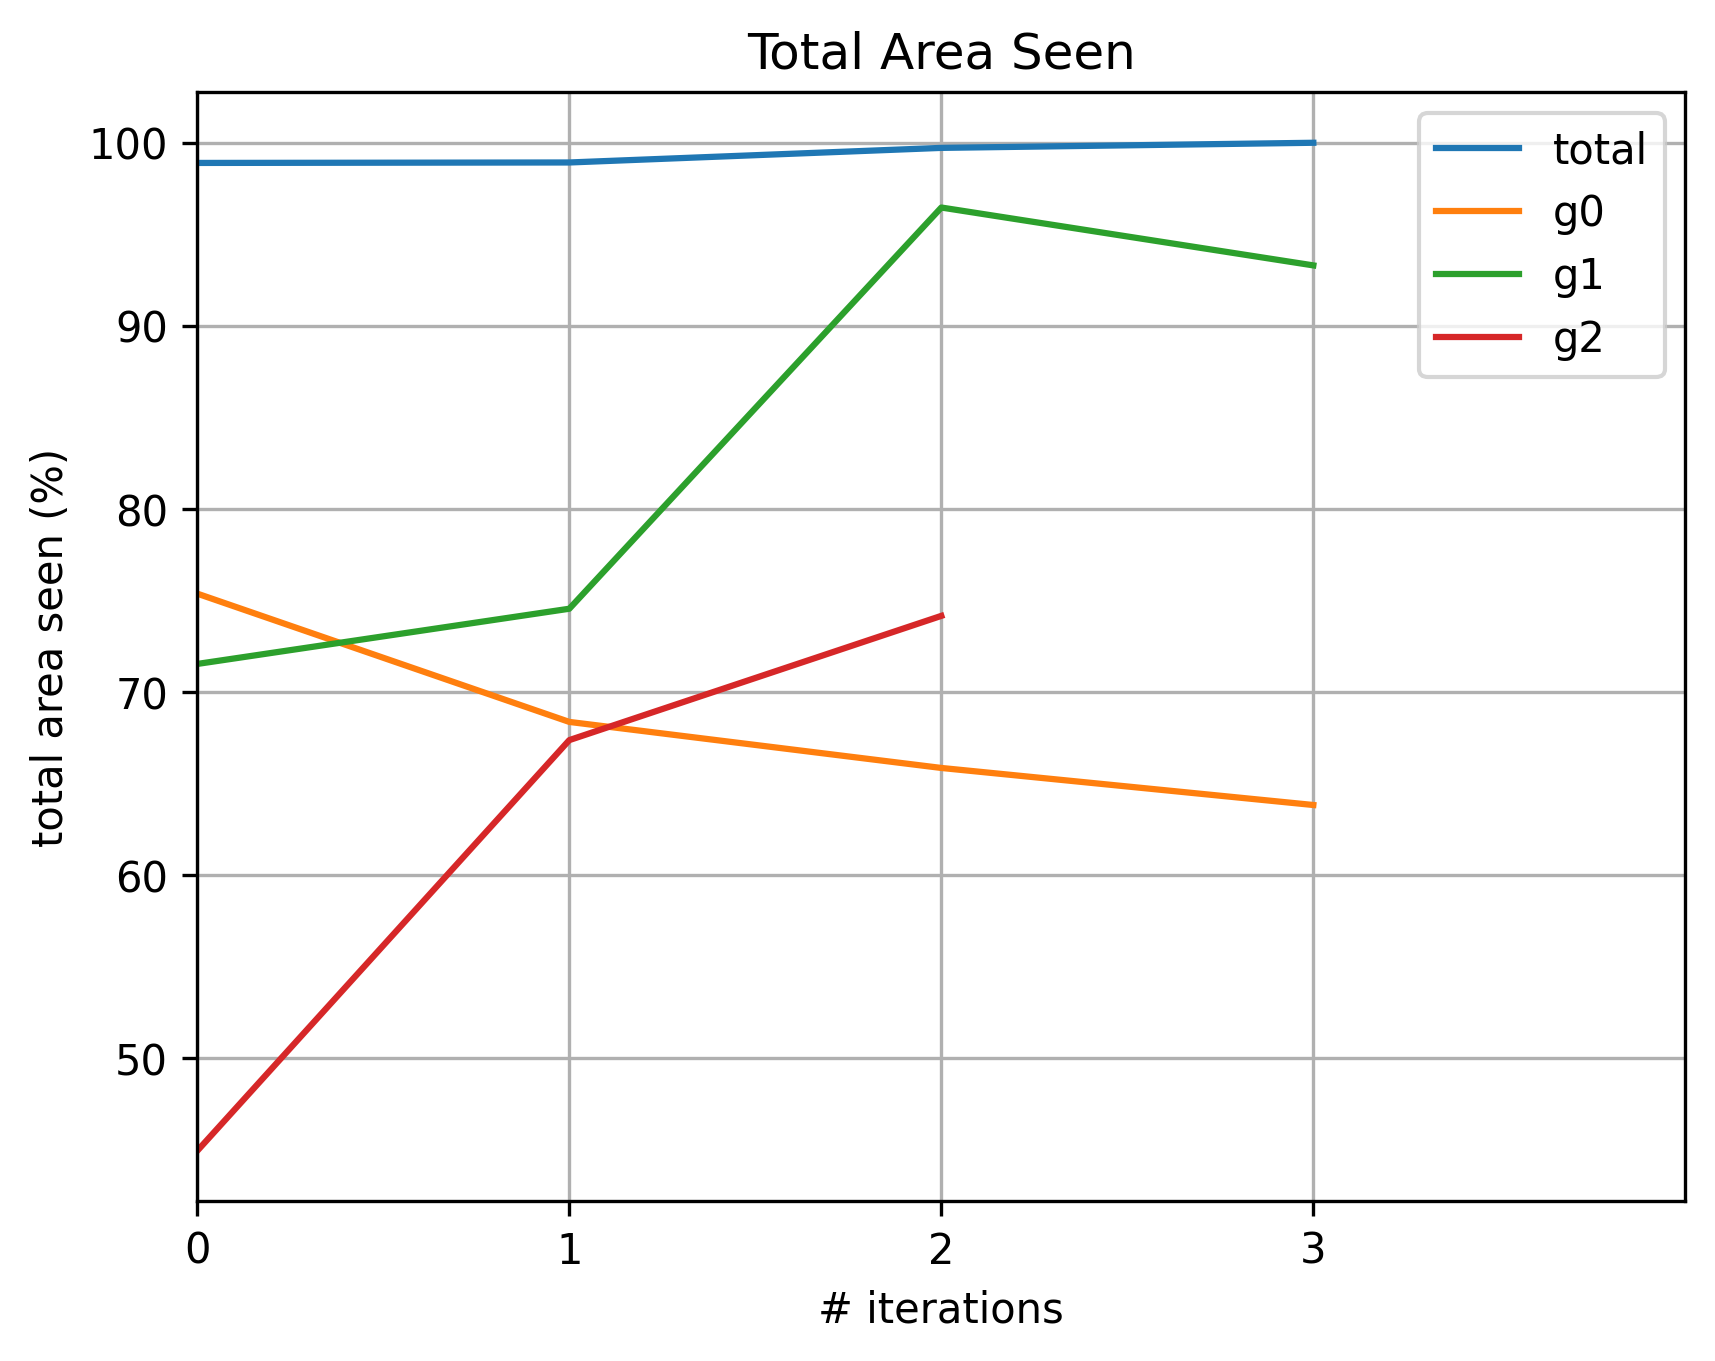
\includegraphics[width = \textwidth]{experiments/area_random_all.png}
        \caption{All heuristics.}
        \label{fig:no_momentum1}
    \end{subfigure}
    \begin{subfigure}{0.45\textwidth}
        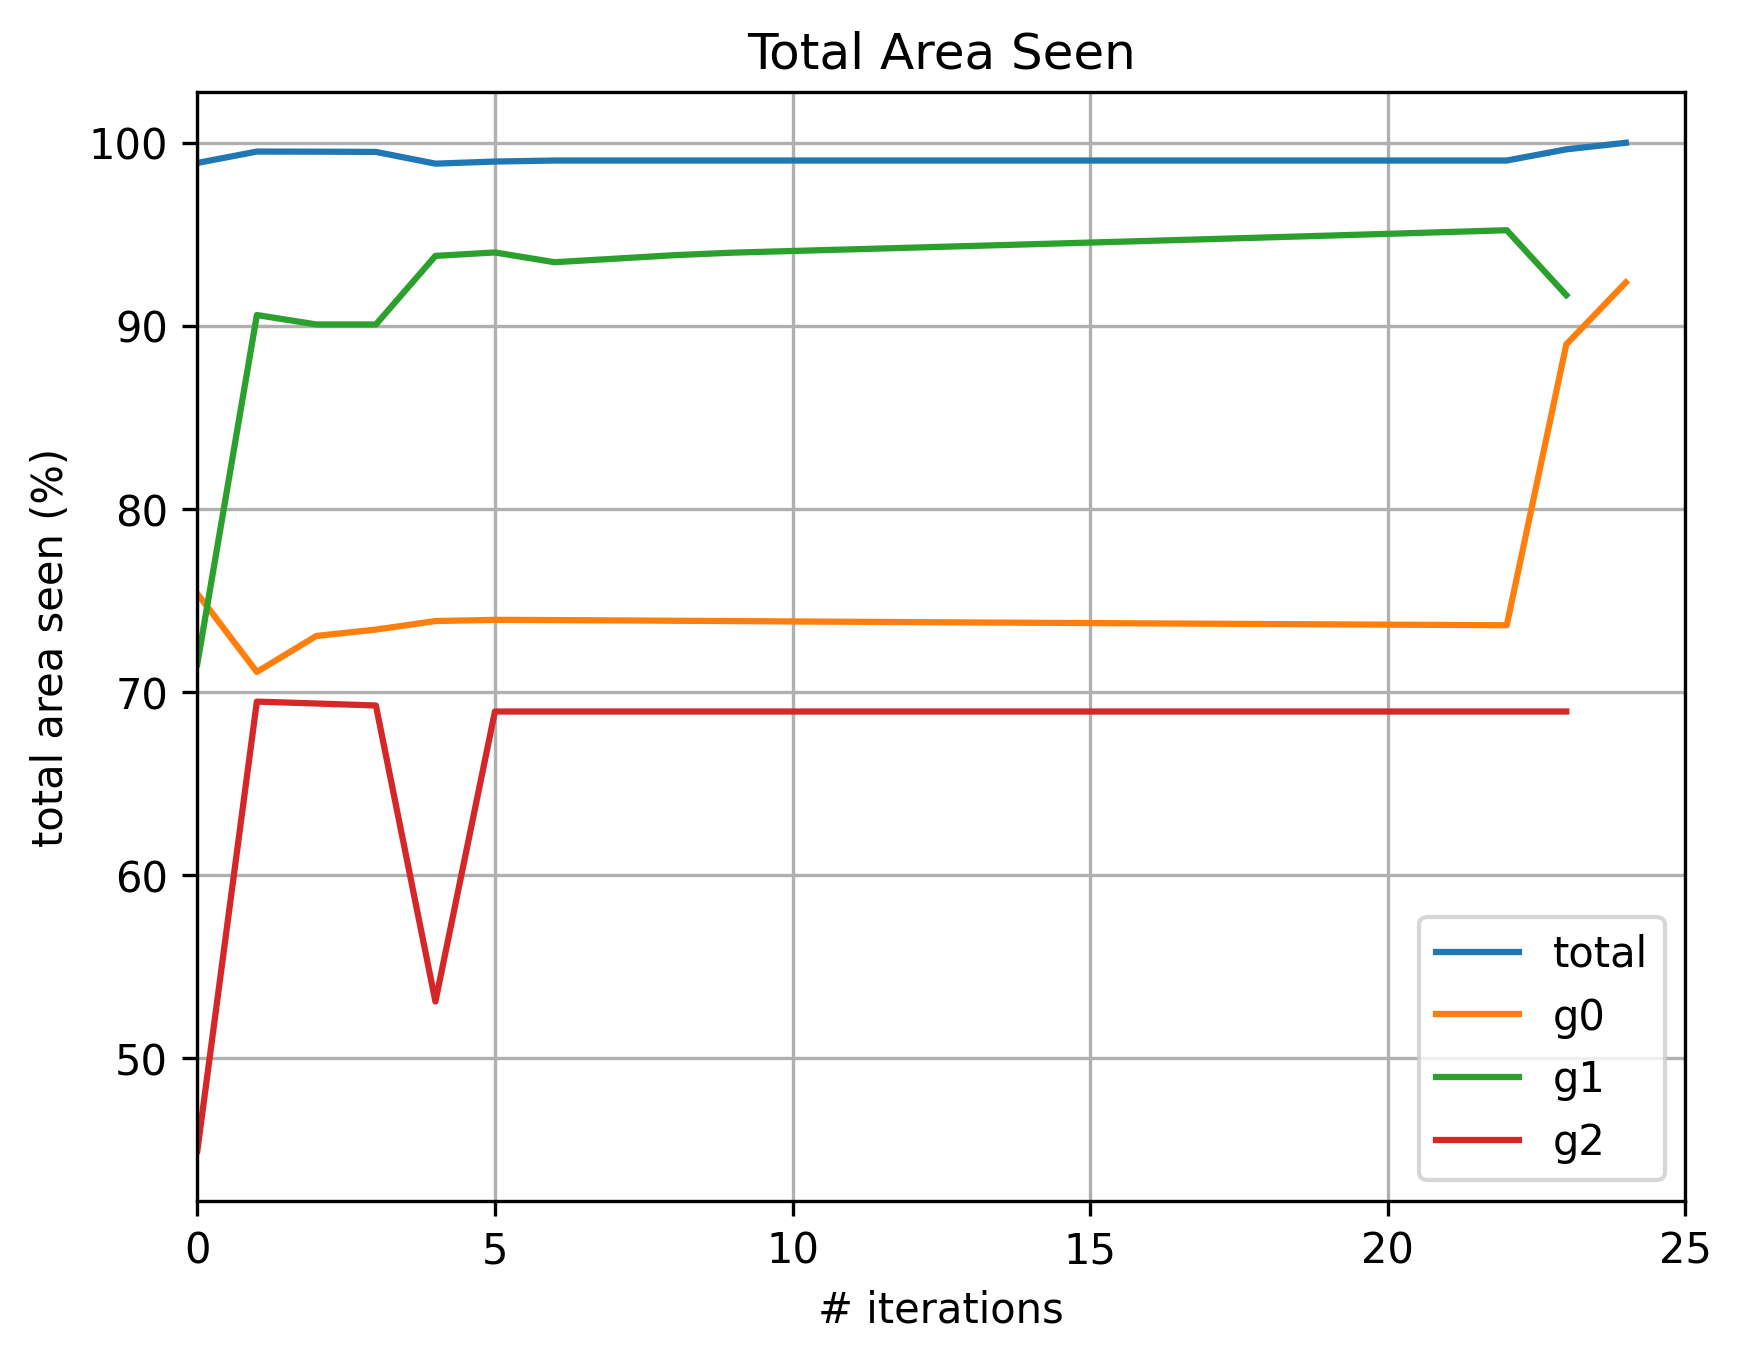
\includegraphics[width = \textwidth]{experiments/area_random_no_momentum.png}
        \caption{No momentum.}
        \label{fig:no_momentum2}
    \end{subfigure}
    \caption{Total area seen per iteration for an arbitrary polygon guarded by 3 guards.}
    \label{fig:no_momentum}
\end{figure}

\subsubsection{Without Line Search}
In this section we will discuss the impact line search has on the overall behaviour of the algorithm. As introduced in Section \ref{sec:line_search}, line search determines how far a guard should move into the optimal direction. In this way, it computes the optimal position of a guard on the direction line given a step size.
In our experiments, the search will compute the best guard placement between multiple positions computed from movement factor $\frac 1 32$ to 32 with a step size $s = 2$.

A suggestive way to observe how well Line Search works is with the comb polygon with four teeth from Figure \ref{fig:comb}.

\begin{figure}[h!]
    \centering
    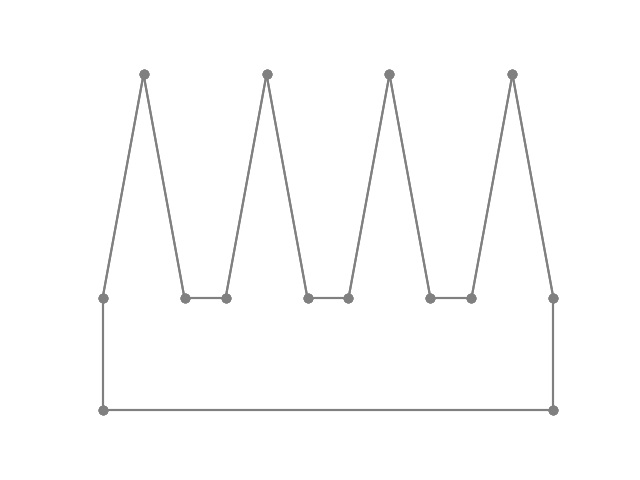
\includegraphics[width = 0.5\textwidth]{experiments/comb.png}
    \caption{Polygon in the shape of a comb with four teeth.}
    % \label{fig:comb}
\end{figure}

We will compare how the guards move when we are using all the heuristics to when we are not using line search. The guards will have a learning rate $\alpha = 0.4$ for the case when line search is used, and $\alpha = 0.6$ for when it is not used. They will start at the same fixed position in both cases.

Figure \ref{fig:no_line_search} displays the area seen per iteration for the comb polygon with four teeth. Both the total area seen and the individual area seen by each guard are shown. Starting with around 82.5\% total area seen, the guards are eventually optimally placed in a position from which the whole polygon is seen. Nonetheless, using line search clearly makes a difference between Subfigures \ref{fig:no_line_search1} and \ref{fig:no_line_search2}. The first noticeable difference is the number of iterations. Using line search allows the guards to find their optimal positions in 3 iterations, with a steady increase in the total area seen. On the other hand, not using line search results in the optimal position to be found in more than 80 iterations. What is more, 3 of the guards seem to have found their optimal position after the $30^{\text{th}}$ iteration, whereas the last 50 iterations are spent on only one guard finding its own.

Therefore, we reckon that line search significantly and more efficiently speeds up the process of finding the optimal position for each guard. In this way, each guard moves faster to its optimal position and avoids creating situations where multiple guards that have found their optimal position have to wait for only one guard to find its own.


\begin{figure}[h!]
    \centering
    \begin{subfigure}{0.45\textwidth}
        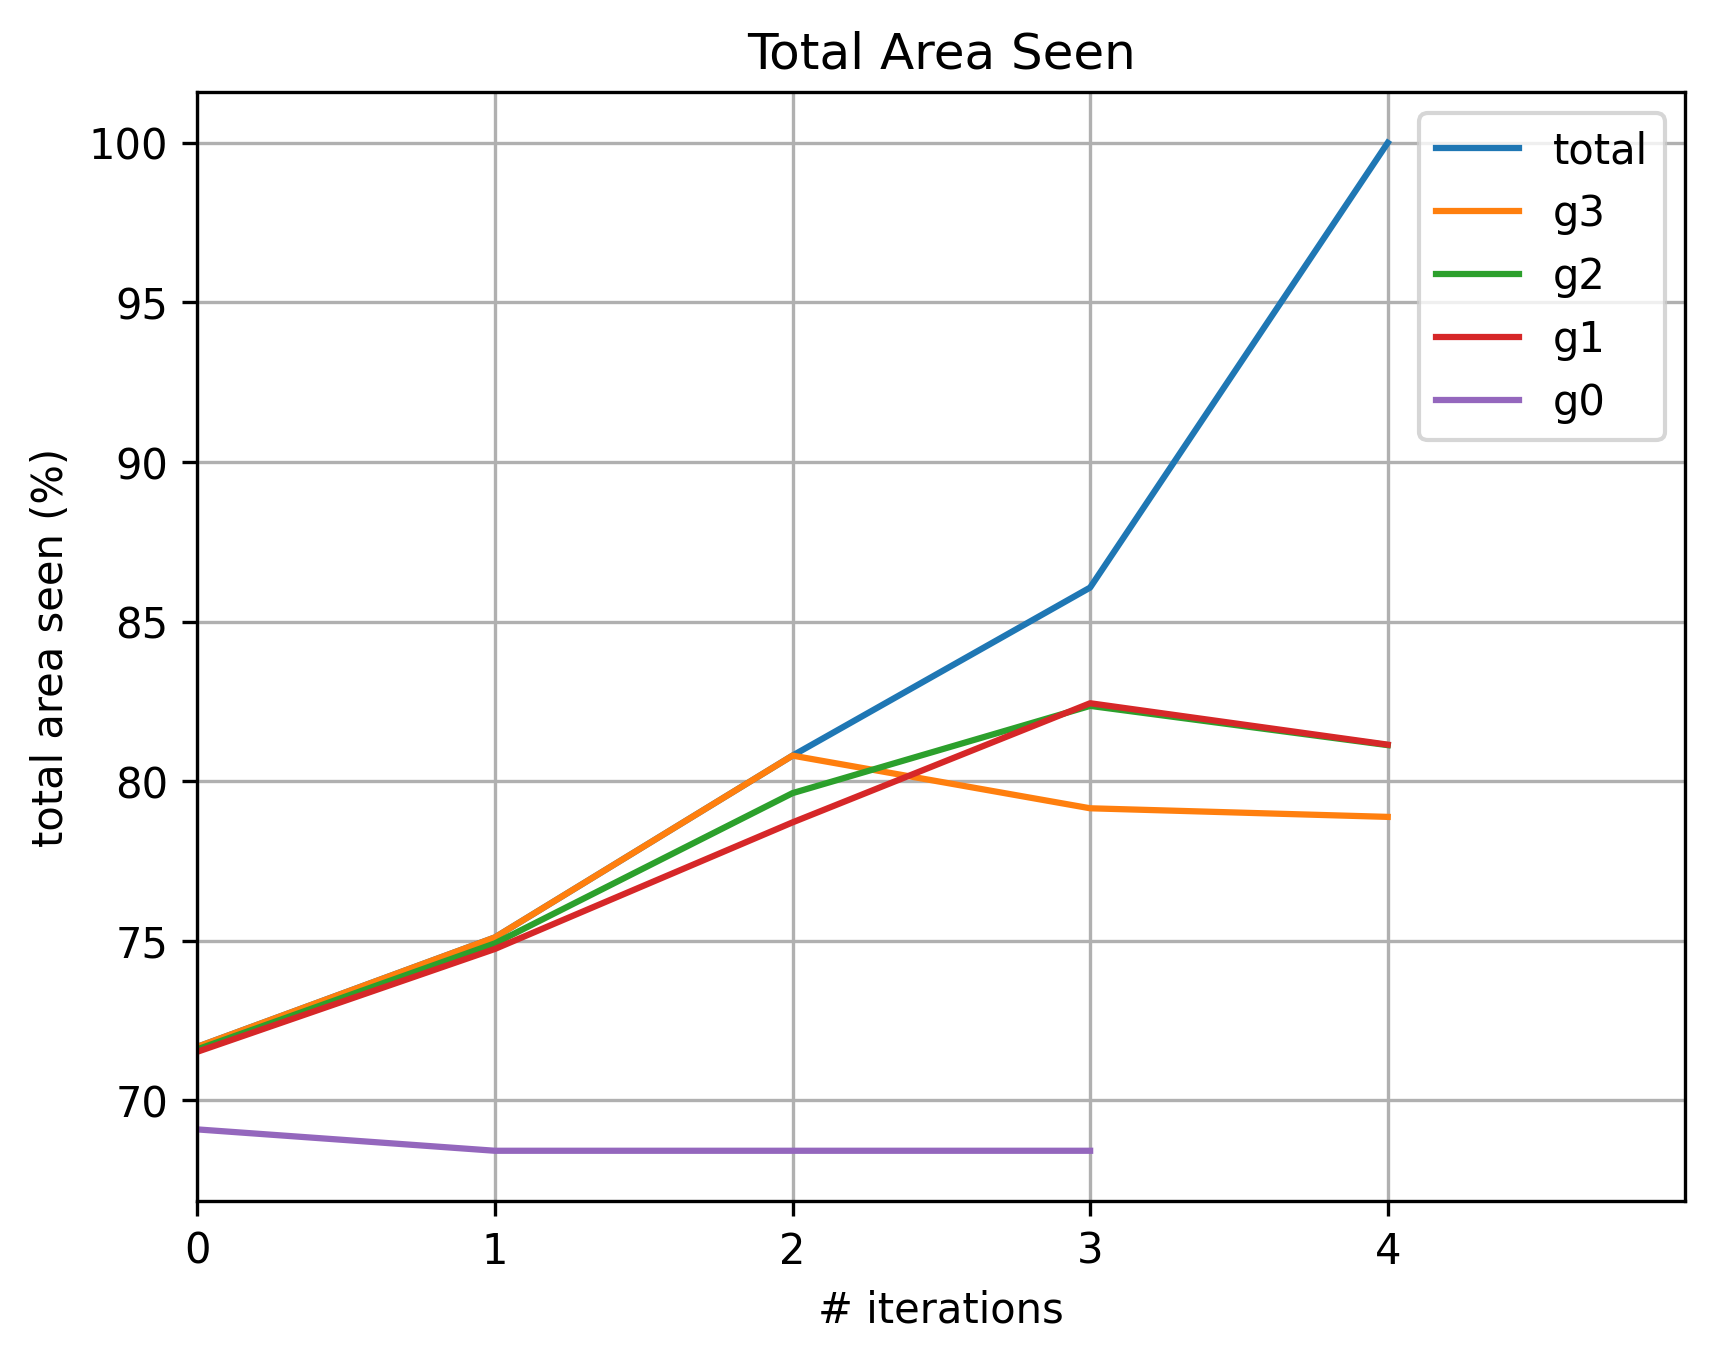
\includegraphics[width = \textwidth]{experiments/area_comb_all.png}
        \caption{All heuristics.}
        \label{fig:no_line_search1}
    \end{subfigure}
    \begin{subfigure}{0.45\textwidth}
        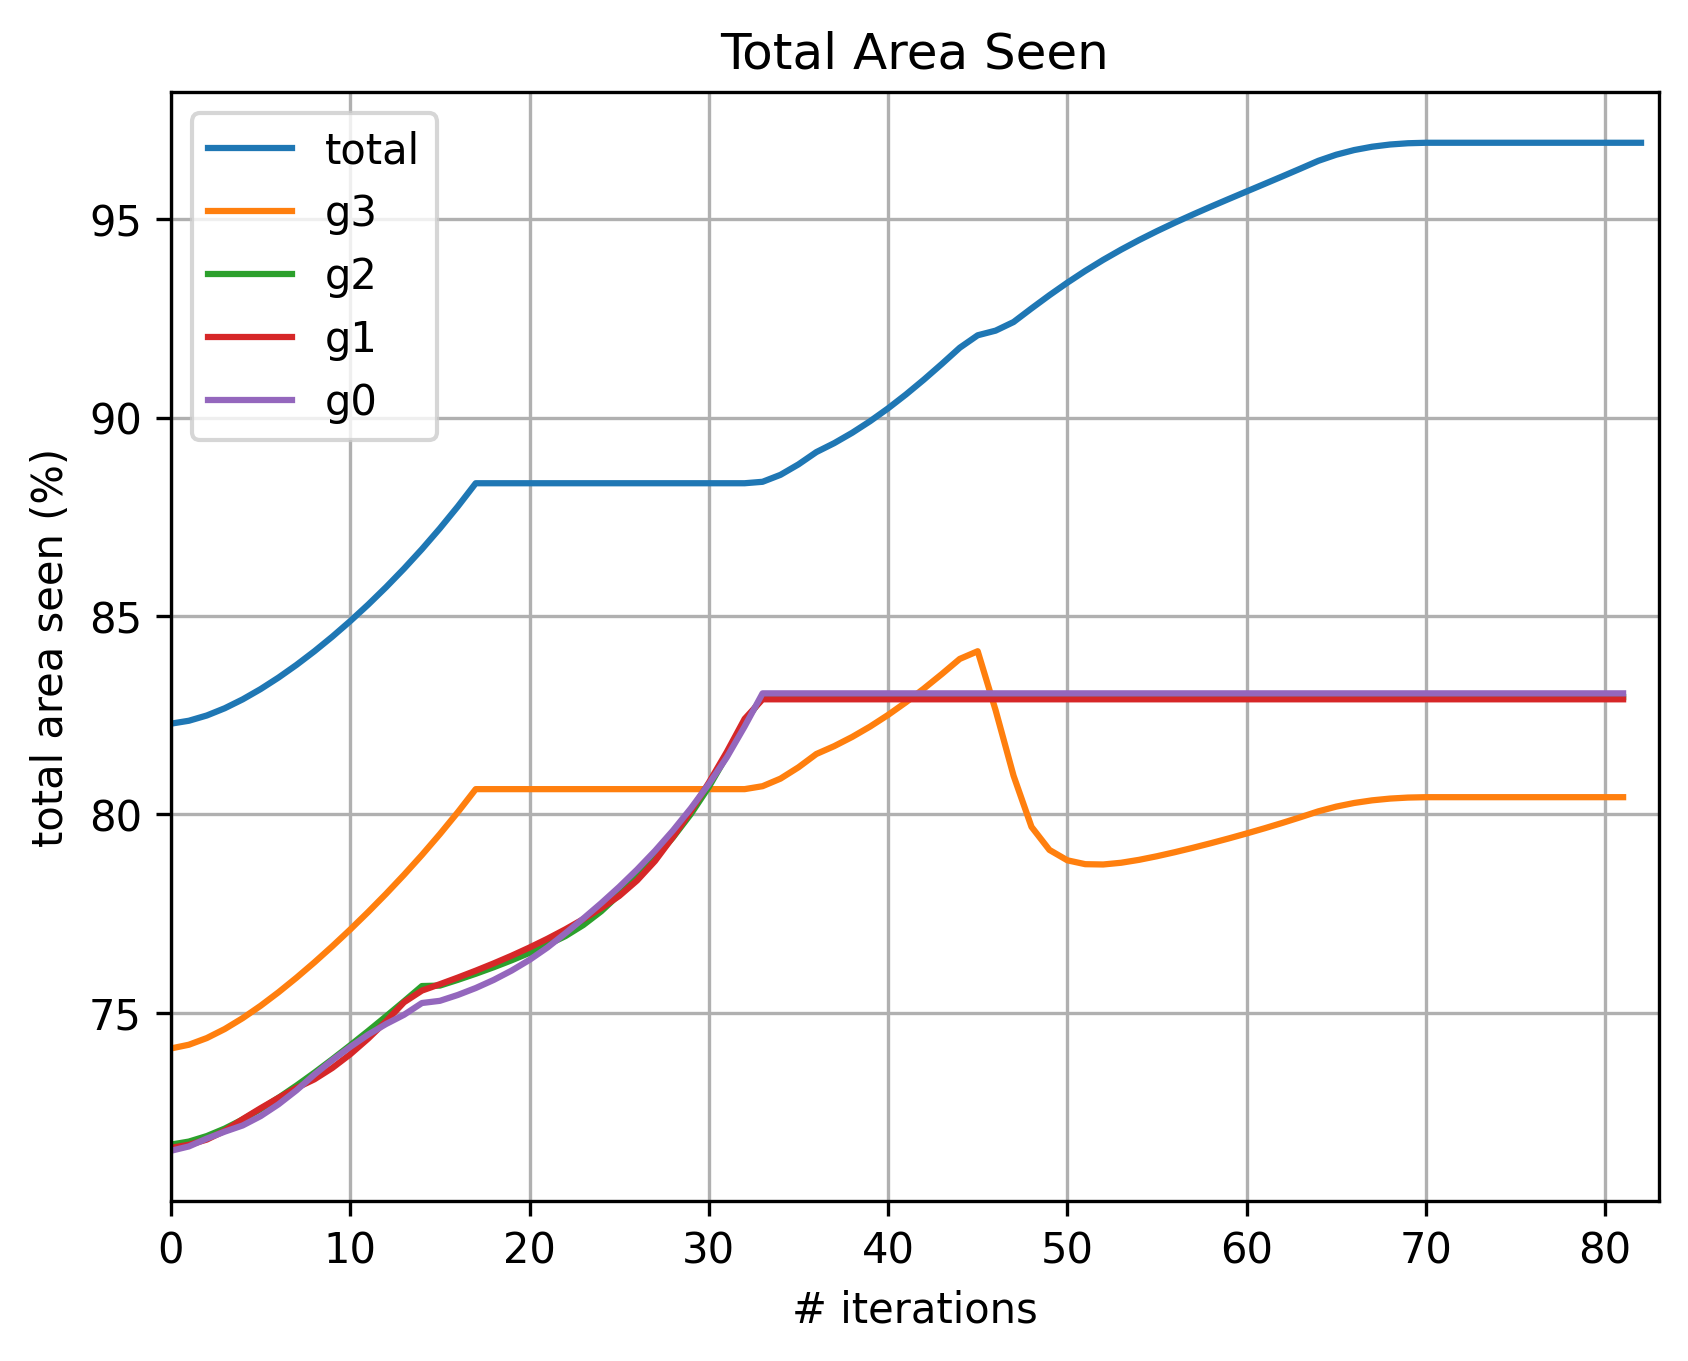
\includegraphics[width = \textwidth]{experiments/area_comb_no_linear_search.png}
        \caption{No line search.}
        \label{fig:no_line_search2}
    \end{subfigure}
    \caption{Total area seen per iteration for the comb polygon with four teeth.}
    \label{fig:no_line_search}
\end{figure}

% - momentum
- reflex vertex pull
    - onto reflex vertex
    - pull Capping
% - line search
- reflex area
- hidden gradient
- angle behind reflex vertex
- greedy initialisation